\documentclass[12pt]{article}

\usepackage[english]{babel}
\usepackage[utf8x]{inputenc}
\usepackage{pdfpages}
\usepackage{lastpage} % Required to determine the last page for the footer
\usepackage{extramarks} % Required for headers and footers
\usepackage{graphicx} % Required to insert images
\usepackage{listings} % Required for insertion of code
\usepackage{courier} % Required for the courier font
\usepackage{color}
\usepackage{grffile}
\usepackage{float}

\usepackage[a4paper, total={6in, 8in}]{geometry}

% Margins
\topmargin=-0.45in
\evensidemargin=0in
\oddsidemargin=0in
\textwidth=6.5in
\textheight=9.0in
\headsep=0.25in
\fboxsep=0mm%padding thickness
\fboxrule=2pt%border thickness

\linespread{1.1} % Line spacing

\newcommand{\Title}{Architecture specification Document} % Assignment title
\newcommand{\Class}{Cos\ 301} % Course/class
\newcommand{\pd}{Post-Doctoral}
\newcommand{\ssr}{Soft\color{green}{Serve }\color{black}}
\newcommand{\version}{1.0}
\newcommand{\iteration}{2}
\newcommand{\client}{Ms. Cathy Sandis (UP Research Office)}
\newcommand{\project}{Post-Doctoral Application Management System}
\newcommand{\repo}{https://github.com/mox1990/Project-Postdoc.git}

\begin{document}


\vspace{4em}

\begin{center}%

\begin{figure}[ht!]
\centering

\includegraphics{../Images_Docs/logo.png}
\end{figure}
\LARGE \bf \project \\[1em]
\LARGE \bf \Title \\[0.25em]
\large \bf \today\\
\bf Version \version\\
\bf Iteration \iteration\\[0.5em]
\Large \bf Prepared for \client\\
\Large \bf by
\Large {\bf \ssr Group }\\[0.5em]
\LARGE {\bf Group members}\\[0.25em]
\large
Kgothatso Phatedi Alfred Ngako (12236731) \\[0.5em]
Tokologo “Carlo” Machaba (12078027) \\[0.5em]
Mathys Ellis (12019837) \\[8em]

\end{center}%

%\newpage
%{\LARGE \bf Change log}\\[2em]

\begin{center}
\begin{tabular}{|l|p{1.4cm}|p{8cm}|p{2.8cm}|}
\hline
\multicolumn{4}{|c|}{\bf Change log} \\
\hline
 Date & Version & Description &  Person \\
\hline
18/05/2014 & v 0.0 & Document created. & Alfred Ngako \\
\hline
19/05/2014 & v 0.1 & Added more detail to information in subsections. & Alfred Ngako \\
\hline
20/05/2014 & v 0.2 & Added references and citations. & Alfred Ngako \\
\hline
22/05/2014 & v 0.3 & Transferred architectural scope to architectural requirements specification document. Began editing. & Mathys Ellis \\
\hline
23/05/2014 & v 0.4 & Added to and edited architectural patterns and style. & Mathys Ellis \\
\hline
23/05/2014 & v 1.0 & Finalised and edited document for first iteration. & Mathys Ellis \\
\hline
18/08/2014 & v 2.1 & Added to technologies as well as updated the section. & Mathys Ellis \\
\hline
%\end{tabbing}
\end{tabular}
\end{center}
\newpage
\tableofcontents

\listoffigures
\newpage
\section{Project Repository}
\textbf{\repo}
\newpage
%%%%%%%%%%%%%%%%%%%%%%%%%%%%%%%%%%%%%%%%%%%%%%%%%%%%%%%%%%%%%%%%%%%%%%%%%%%%%%%%%%%%%%%%%%%%%%%%%%%%%%%%%%%%%

\section{Document description:}%Not entirely sure what I should add here

\subsection{Document purpose}
\vspace{0.2in}

This document follows on the Architecture requirements specification document. The Architecture specification document provides the architectural descriptions of various architectural factors that the project will need to follow when developing the system.  Architecture in this document's context refer to the technological basis and software development styles of the project. Thus this document serves as a contract between SoftServe and the client, Mrs Cathy Sandis of the DRIS of the University of Pretoria in terms of what technologies the project should incorporate as-well the software development infrastructure that the system will be based on.
\vspace{0.2in}

\subsection{Documentation methodology}
\vspace{0.2in}
\begin{flushleft}
The documentation and software development methodology used by the project adhere to the guidelines set out by the scum agile methodology. Thus this document has undergone and will undergo various iterations that may extend or reduce the contents of the document.\\

The document was compiled using a software architecture specification document template provided by Dr Fritz Solms as an alternative to the Kruchten 4 + 1 approach to documenting software.

This document was created using the requirement elicitation techniques and requirement definitions as specified by Klaus Pohl’s book Requirements Engineering: Fundamentals, Principles, and Techniques [Dr.Phol, K., 2010].
The requirements, vision and scope were elicited from the following sources:
\begin{itemize}
	\item Numerous interviews with the client.
	\item On-line research into UP Post doctoral applications.
	\item Correspondence with the UP IT department.
	\item Collecting and analysing various documents such as:
		\begin{itemize}
			\item The initial project request document
			\item Application forms
			\item Renewal forms
			\item CV templates
			\item Approval and recommendation forms
		\end{itemize}
\end{itemize}
\end{flushleft}	

\vspace{0.5in}

\subsection{Document conventions:}
\vspace{0.1in}
\begin{itemize}
\item Documentation formulation tool: LaTeX
\end{itemize}

\vspace{0.2in}

\subsection{References:}
\vspace{0.1in}
\begin{itemize}
\item Kang, A. August 9, 2002, \textit{Enterprise application integration using J2EE}, Available from: http://www.javaworld.com/article/2074488/enterprise-java/enterprise-application-integration-using-j2ee.html , [Accessed on: 17 May 2014]
\item Ali Babar, M., \textit{Architectural Patterns and Frameworks, Week 3, Lecture 3},Available from: https://blog.itu.dk/MSAR-E2013/files/2013/09/wk3\_lect3\_patternsframeworktactics.pdf, [Accessed on: 21 May 2014]
\item Dr.Phol, K., 2010, \textit{Requirements Engineering: Fundamentals, Principles, and Techniques}, Springer, Heidelberg.
\item Kayal, D., 2008, \textit{Pro Java EE Spring Patterns: Best Practices and Design Strategies Implementing Java EE patterns with Spring Framework}, Apress, New York.
\item Jendrock E, Cervera-Navarro R, Evans I, Haase K, Markito W, \textit{The Java EE 7 Tutorial}, Available from: http://docs.oracle.com/javaee/7/tutorial/doc/home.htm , [Accessed on: 20 May 2014]
\item Oracle. April 2014, \textit{The Java EE 7 Tutorial}, Available from: http://docs.oracle.com/javaee/7/tutorial/doc/overview.htm , [Accessed on: 20 May 2014]
\end{itemize}	

\vspace{0.5in}

\newpage

%%%%%%%%%%%%%%%%%%%%%%%%%%%%%%%%%%%%%%%%%%%%%%%%%%%%%%%%%%%%%%%%%%%%%%%%%%%%%%%%%%%%%%%%%%%%%%%%%%%%%%%%%%%%%
\section{Architecture Requirements} 
This section can be found in the architecture requirements specification document in which it discusses the following:
\begin{itemize}
\item Architectural scope
\item Access channel requirements
\item Quality Requirements
\item Integration requirements
\item Architectural Constraints
\end{itemize}

%%%%%%%%%%%%%%%%%%%%%%%%%%%%%%%%%%%%%%%%%%%%%%%%%%%%%%%%%%%%%%%%%%%%%%%%%%%%%%%%%%%%%%%%%%%%%%%%%%%%%%%%%%%%%


\section{Architectural Patterns and Styles} % skipped till further notice.

% Mention of how Java EE actually doesn't require use of GoF design patterns >> http://www.theserverside.com/tip/With-Java-EE-7-your-Design-Patterns-are-dead-And-your-EAR-is-ugly-too <<

The system will employ the Model-View-Controller, MVC, architectural pattern combined with a multi-tier/layered architectural pattern to form what is known as the Java Enterprise Edition system architecture. This will allow the client(s) to be decoupled from the server. Further this allows the view, the controller and the model each to have its own set of layers. Both of these patterns provide various benefits and are widely used. Some benefits include modularity, encapsulation, re-usability of components, decoupling and system maintainability [Ali Babar, M.] [Oracle, 2014][Kayal, D., 2008]\\
\\
The Java EE system architecture is designed to support highly scalable, distributed, transactional, and portable applications that use the speed, security, and reliability of a Java EE server to provide powerful enterprise applications. [Oracle, 2014] For this reason SoftServe believes this system architecture is well suited for the development of the Post-Doctoral application management system as it will satisfy the requirements in terms of quality and functional as stipulated by the client. The following diagram provides the system architectural that will be employed by the system:\\

\begin{figure}[H]
\centering
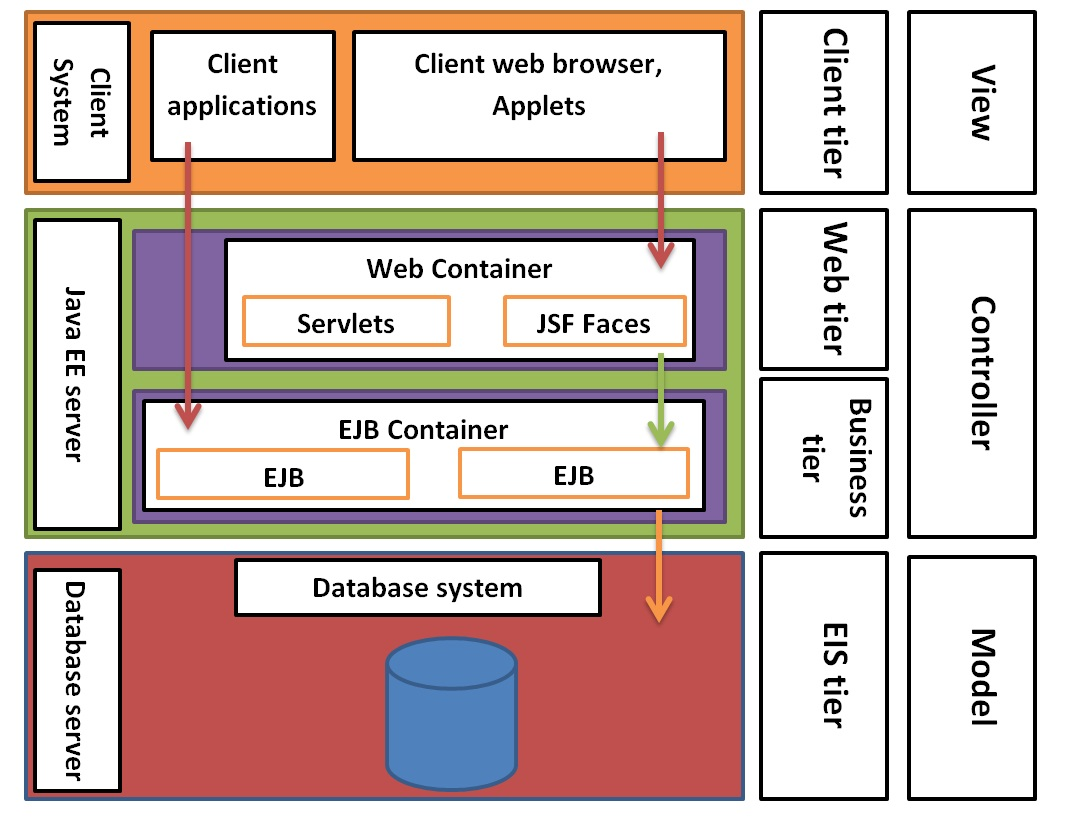
\includegraphics[scale=0.8]{../Images_Docs/Diagrams/Architecture/Java EE system architecture.jpg}
\caption{Java EE system architecture}
\end{figure}

\subsection{View}
The View component of the system architecture is used to represent and encapsulate the front-end of the system. It contains the client tier of the Java EE system architecture. Thus this allows the system to decouple the front-end and the back-end components. Allowing various clients to access the back-end without having to duplicate certain back-end tiers for each client. [Kayal, D., 2008]
\subsubsection{Client Tier}
This tier runs on the client system and encapsulates the various components that a client system may use to access the Java EE server-side tiers. These components include dynamic web pages, Java applications and Java applets. In order to make the Post-doctoral application management system accessible to any stakeholder over the internet and provide a uniform user experience the system will only make use of the dynamic web pages component provided by the Java EE client tier. [Oracle, 2014]  
\subsection{Controller}
The controller component of the system architecture is used to provide the business logic and manage and manipulate the view's request in order to provide communication between the Model component and the View. This component therefore hosts the web tier and the business tier of the Java EE application. This component is located on the Java EE server which is a multi-threaded application server. [Kayal, D., 2008] [Oracle, 2014] 
\subsubsection{Web Tier}
This Tier runs on the Java EE server and hosts the Web container. It provides the management and web page generation support for the web pages that the system has to provide to the view through the user of servlets, Java ServerPages and Java ServerFaces Facelets. Facilitates the communication between the business tier and client tier for web browser clients and applets. Client applications do not have to make use of the Web Tier and can directly skip to the business tier. But as stipulated above the other types of client components will not be considered for the project. [Oracle, 2014]
\subsubsection{Business Tier}
This Tier also runs on the Java EE server and hosts the Enterprise Java Bean container. It provides the business logic section for the Java EE application in the form of Enterprise Java Beans which are simply classes that represent various persistence entities of the data base, system messages, sessions, etc. This tier communicates with EIS tier in order to get access the database and various other lower level infrastructures that the Java EE application requires. [Oracle, 2014]
% More bullshit goes here.
\subsection{Model}
The Model component of the system architecture contains the various persistence storage infrastructure and lower level system management features such as transaction processing. It hosts the Enterprise Information System tier of the Java EE application. [Kayal, D., 2008]
\subsubsection{Enterprise Information Tier} 
The EIS tier provides mainly the support for database systems that is used by the Java-EE application. This tier can run on the Java-EE server as a virtual server or on a physically different database server. Due to the project budget and technical constraints the former will used by the system. [Oracle, 2014] 
 
%%%%%%%%%%%%%%%%%%%%%%%%%%%%%%%%%%%%%%%%%%%%%%%%%%%%%%%%%%%%%%%%%%%%%%%%%%%%%%%%%%%%%%%%%%%%%%%%%%%%%%%%%%%%%
\section{Architectural Tactics and Strategies} % skipped till further notice.
This section describes the architectural techniques which will be used in order for the system to satisfy the quality requirements. 

% This section needs a lot of paraphrasing...
\subsection{Concurrency}
The Java Platform has always offered support for concurrent programming, which is the basis for implementing many of the services offered by Java EE containers. This is realized through the two main concepts of having a multiple threads execute under a single process, in the case of Java EE mulitple beans execute under the JVM. The number of threads that can execute under the JVM can go well beyond thousands depending on factors such as the machine the JVM is running on and how it has been configured.\\

Even though the concurrent threads will mean better performance and a scalable implementation for the system they may lead to issues that effect the reliability and integrity of the system such as:
\begin{itemize}
\item Deadlocks,
\item Thread Starvation,
\item Concurrent  accessing of shared resources, and
\item Situations where the program generates incorrect data.
\end{itemize}

To deal with these issues Java EE provides concurrent utilities that access concurrent resources via JNDI lookup or resource injection. The components in the utilities ensure that the issues mentioned above are nullified. The primary components of interest in the concurrent utilities for our system are:
\begin{itemize}
\item managed executor service, 
\item managed scheduled executor service, 
\item managed thread factory, and 
\item context service.
\end{itemize}
\subsubsection{Concurrency Utilities for Java EE}
\subsubsection{Managed Executor Service}
A managed executor service is used by applications to execute submitted tasks asynchronously. Tasks are executed on threads that are
started and managed by the container. The context of the container is propagated to the thread executing the task.

For example, by using an ManagedExecutorService.submit() call, a task, such as the GenerateReportTask, could be submitted to execute at a later time and then, by using the Future object callback, retrieve the result when it becomes available ().

\subsubsection{Managed Scheduled Executor Service}
A managed scheduled executor service is used by applications to execute submitted tasks asynchronously at specific times. Tasks are executed on threads that are started and managed by the container. The context of the container is propagated to the thread executing the task. The API
provides the scheduling functionality that allows users to set a specific date/time for the Task execution programmatically in the application.

\subsubsection{Managed Thread Factory}
A managed thread factory is used by applications to create managed threads. The threads are started and managed by the container. The context of the container is propagated to the thread executing the task. This object can also be used to provide custom factories for specific use cases (with custom Threads) and, for example, set specific/proprietary properties to these objects (Cervera-Navarro, Evans, Jendrock, Haase and Markito 2014).

\subsection{Builder Pattern}
The Builder Design Pattern allows for the construction of complex structures in small steps. An example of how it is used is in the process of making an application, the different elements of an application are separated. The process of creating objects speeds up as well. This construction of objects in small steps decreasing coupling and makes the code more testable. The design helps improve the flexibility as well as the maintainability of the code.  

\subsection{Factory Design Pattern}
The Factory Design Pattern provides centralised to create our Database entities and entries in an orderly fashion. The pattern allows the developers to define an interface for creating an object, but let the classes that implement the interface decide which class to instantiate. By doing this the code is now flexible and creation of new objects is much simpler. It also helps redundancy 

\subsection{State Design Pattern}
The State Design Pattern is best used in situations where the actions take place in a pre-defined order as with this project. The State pattern changes the state of the objects depending on how far in the pipeline. It provides a simple and clean way to change the state of an object during run time. The design pattern improves the usability of the system as users will know exactly when some change has taken place. 

\subsection{Dependency Injection}
This is used to implement, inversion control. The client is only allowed to use a service rather than creating their own services. The design pattern allows a client to remove all knowledge of a concrete implementation that it needs to use. This helps isolate the client from the impact of design changes and defects. It promotes re-usability, testability and maintainability 

\subsection{Database Access Objects}
The Database Access Object is used by all the application calls to provide specific data operations without exposing details of the database to external objects. It forms part of the Core J2EE Patterns. This design pattern acts an intermediary between the application and database, by moving back and forth between objects and database records. It also contains the effects of any changes to the persistence mechanism to a confined area and not the whole application. This pattern improves the audit-ability as well maintaining the integrity of the data contained in the system. 

The use of DAO will help reduce the existance of object-relational impedance mismatch present in the system. It will also contribute to the flexibilty of the system. In the case where the systems underlying persistance mechanism has to change only the DAO will have to be updated and all the places in the system where the DAO was used will then remain constant.

%%%%%%%%%%%%%%%%%%%%%%%%%%%%%%%%%%%%%%%%%%%%%%%%%%%%%%%%%%%%%%%%%%%%%%%%%%%%%%%%%%%%%%%%%%%%%%%%%%%%%%%%%%%%%
\section{Use of Reference Architecture and Framework}
The core design philosophy of the Java-EE platform is to provide a Java-EE application developer with a set of test and well maintained and reusable APIs as well as frameworks that allow them to focus rather on implementing the actual business logic and UI than focusing on the underlying system technical and management services such as authentication, session management, etc. Thus the Java EE platform provides a runtime environment for developing and running large-scale, multi-tiered, scalable, reliable, and secure network applications. As seen above it also provides a system architecture and various frameworks, discussed below, for implementing services for multi-tier applications that deliver the scalability, accessibility, and manageability needed by a system. Taking all the above into consideration this makes it ideal for the development of the project.

\subsection{JavaServer Faces (JSF)}
JSF is a web application GUI framework that is based on the JSP, EL and servlet technology that Java-EE provides. It allows the generation of various mark-up languages, such as HTML 4.0.1 and HTML 5, directly from objects and ORM model objects used by the Java-EE application. Thus it is ideal for system as the system needs to provide support for both HTML 5 and 4.0.1 web content.\\

It will help achieve the usability quality requirement as it will implement all aspects of the user interface.

\subsection{Java Persistence API}
Java EE is based on Java which is an object-oriented language. Whereas most modern day database management systems, DBMSs, provide relation databases. Thus to bridge this gap the Java Persistence API is used. It provides a Object Relational Mapping solution which allows the relation database to be viewed as a object-oriented database. Thus this critical for the system SoftServe wishes to develop as the system will make use of MySQL which is a relation database management system. The Java persistence API contains the following components:  
\begin{itemize}
\item Persistence API
\item The query language
\item ORM
\end{itemize}
\subsection{Java API for RESTful Web Services (JAX-RS)}
The JAX-RS API provides a way for the Java-EE application to provide web services or data transfer via the HTTP or HTTPS protocol using the Representational State Transfer, REST, architectural style. This accomplished by the user of various JAX-RS runtime annotations. This will allow the system to provide a set of lightweight web services to various clients across the internet. This will allow the system to easily be accesses by mobile and computer platforms alike and also be accessible over most companies firewalls as it will make use of the HTTPS protocol. Further this will allow for future expansion if client wishes it. To insure security a the POST command will be preferred above GET.[Cervera-Navarro, Evans, Jendrock, Haase and Markito, 2014]
\subsection{JUnit}
JUnit is a simple unit testing framework used to write repeatable tests. Test methods must be annotated by the @Test annotation. It is also possible to define a method to execute before (or after) each (or all) of the test methods with the @Before (or @After) and @BeforeClass (or @AfterClass) annotations. \\

It will be used to achieve the testbility of the system.
%\subsubsection{Java EE Connector Architecture}
%%%%%%%%%%%%%%%%%%%%%%%%%%%%%%%%%%%%%%%%%%%%%%%%%%%%%%%%%%%%%%%%%%%%%%%%%%%%%%%%%%%%%%%%%%%%%%%%%%%%%%%%%%%%%

\section{Access and Integration channels}
This section discusses the requirements for the access channels through which the system can be accessed by humans and other systems. Also it discusses the integration channels which need to be used by the system. 

\subsection{Access Channels}
To provide a system that is as accessible as possible the system provide its services through this essentially makes the system OS independent and accessible over firewalls since it will make use of the HTTPS protocol that is usually not blocked by firewalls. This also improves the usability the system as most computer user or mobile users are aware of how to use web browsers. The system will support the following versions of modern web browsers for both their computer and mobile counterparts:
\begin{enumerate}
\item Mozilla Firefox 20+
\item Google Chrome 30+
\item Microsoft Internet Explorer 9+
\item Apple Safari
\item Opera
\end{enumerate}

\subsection{Integration Channels}
As mentioned in the architecture requirements specification document the IT department of the University of Pretoria will only be willing to provide the SoftServe group with the knowledge of the Peoplesoft system in order to integrate it. Thus the SoftServe group will attempt to accommodate the PeopleSoft system as much as possible by conforming to same user name styling, export of data to formats that are used by the Peoplesoft system to import data. Also the since Peoplesoft is an Oracle enterprise system it would have been developed using Java-EE and the Java programming language. This is therefore a strong motivation for Java-EE to be used by the SoftServe group as a development platform for the system. So to allow integration at a more technical level. Though if the integration was to be done this would be done via the EIS teir using the Java EE Connector Architecture API and the JAX-WS API.  


%Upon successful complementation the system must be integrated able with the University of Pretoria's PeopleSoft system. Therefore it is sensible to implement the system in Java EE as it is one of the many components that form part of the multiple tiers that build up  PeopleSoft. \\

%The use of build tools such as Maven will provide a central piece of information with regards to the projects build, reporting and documentation. This central point of information will assist in the integration phase since it is implemented through a standardised build approach which can come into play at a later time through the use of EAI.\\

%The EAI will be achieved via  the logical integration architecture of Direct point-to-point integration (Kang, 2002). This means that the application management system will make direct JDBC calls to the universities databases tables (which needed to be setup to cater for our system at that point). The Integration method will be pushed-based data-level integration (or if all else fails UI-Level integration).
% http://www.javaworld.com/article/2074488/enterprise-java/enterprise-application-integration-using-j2ee.html

\section{Technologies}
This section discusses and elaborates on the technologies that the system will use and should also be seen as an extension of the architectural constraints, specified in the Architecture requirements specification document, in terms of elaboration.

\subsection{Integrated Development Environment}
The system should be buildable independent of an IDE but it will be developed on Netbeans 8.0 to allow for uniformity amongst the development team, with regards to coding style, and provide easy integration with the tools that will be used such as Javadoc, to generate  API documentation in HTML format.

\subsection{Development technologies}
\subsubsection{Java Servlet Technology}
\textbf{Description}\\
A Java servlet is used to extend the Java-EE application server to support HTTP or HTTPS requests and responses. It allows the server to provide RESTful based web services to connecting clients. Thus it acts as a middle man between any HTTP or HTTPS client and the business tier. This will not be used directly but will be used the JSF framework.\\\\
\textbf{Reasons for use}\\
The JSF framework uses servlets to render JSF pages to HTML and provide them to clients connecting via HTTP or HTTPS. Secondly this will allow the solution to provide lightweight RESTful based web services that will help improve accessibility and availability of the solution. Further it will allow the solution to satisfy the access channel requirements.

\subsubsection{JavaServer Pages (JSP)}
\textbf{Description}\\
JSP is a technology that is used by the Java-EE platform to provide a native language approach to creating web pages. It uses HTML or XML to specify static content on a web page and Expression Language (EL) to provide dynamic content. This will not be used directly but will be used by the JSF framework.\\\\
\textbf{Reasons for use}\\
JSF pages is the a specialised version of JSP pages thus it is used in the JSF framework. Secondly it will help with the maintainability of the code as pages based on JSP technology are easily understandable and readable due to the simplicity of the HTML and XML mark-up languages.    
 
\subsubsection{Expression Language (EL)}
\textbf{Description}\\
It is a language used by JSP and JSF pages to write servlet based code snippets which allow the usage of the data available to the servlet to do calculations, call functions, get or set data. The language closely resembles the Java Language syntax.\\\\
\textbf{Reasons for use}\\
It is used by the JSP technology and JSF framework for dynamic content specification and communication with the backing servlet.

\subsubsection{JavaMail API}
\textbf{Description}\\
The JavaMail API provides a robust and well tested email communication infrastructure for any Java based applications.\\\\
\textbf{Reasons for use}\\
This technology will be employed by the system in order to provide the functional email notification infrastructure requirement needed by the solution.

\subsubsection{JavaBeans Activation Framework (JAF)}
\textbf{Description}\\
The JavaBeans Activation Framework allows the Java-EE application to determine the data type of some section of data and thus allow the application to provide access to it by encapsulating it and determining the operations that the application may perform on it.\\\\
\textbf{Reasons for use}\\
This technology is used by the JavaMail API thus it will be used by the system. 

\subsubsection{Java Database Connectivity API (JDBC)}
\textbf{Description}\\
The Java Database Connectivity API provides the a Java-EE application with the means to access data from various datasources including databases, spreadsheet, etc via the Java programming language.\\\\
\textbf{Reasons for use}\\
The system will use this to communicate with the databases located in the EIS tier of the system in order to retrieve and store data in the databases. 

\subsubsection{Java Transaction API (JTA)}
\textbf{Description}\\
The Java Transaction API provides the Java-EE Application with the means to handle and demarcate data transactions to the database. The API allows the the manual or automatic demarcation of database transactions and ensures that the database and ORM entities are synchronised after commits.\\\\ 
\textbf{Reasons for use}\\
This will be used in the system to improve the centralisation and accuracy of the data accessed by users. Further it will be used to allow access to multiple databases located in the EIS tier and the controlling of such resources.

\subsubsection{Enterprise JavaBeans (EJB)}
\textbf{Description}\\
The Enterprise JavaBeans is a component used by all Java-EE applications to encapsulate the various business logic of the application into reusable modules. Thus it contains the attributes and methods associated with the business logic module and hence can be treated as an stand alone unit that can be reused. The two primary EJBs are Session beans that represent a clients session and the data associated with it and a Message-driven bean that can a allow the component to receive messages asynchronously via event listeners. The system will make use of Stateless session EJBs in order to capture the back end services of the solution.\\\\
\textbf{Reasons for use}\\
The use of EJBs will ensure the modularity of the system and the re-usability of its components. Also within the Java-EE framework it is considered the core of the business tier and thus will be required.
  

\subsubsection{Java Naming and Directory Interface (JNDI)}
\textbf{Description}\\
The Java Naming and Directory Interface provides Java-EE applications with the ability to search for data across LDAP, DNS, etc, directory services. Above this it also allows the application to search for objects that exist within the application and provides access to them so that they can be used by the application. It is also used by Java-EE applications to locate object instances of EJBs and managed beans for usage by the application.\\\\
\textbf{Reasons for use}\\
This technology is a core service required by Java-EE applications to function and thus is needed by the solution.

\subsubsection{Java Architecture for XML Binding (JAXB)}
\textbf{Description}\\
JAXB is used to parse any XML data into a set of XML usable Java object instances that represent the content of the XML data. Likewise it is used to convert such objects to XML formatted data. This is accomplished by using an XML schema to define the structure or annotated classes.\\\\
\textbf{Reasons for use}\\
This will be used by the system to handle any XML data extraction or creation from or for storage.

\subsubsection{Jasper Reports}
\textbf{Description}\\
The Jasper reporting library provides a flexible, well-tested and maintained reporting framework to create reports based on data that is located in various data sources.\\\\
\textbf{Reasons for use}\\
This will be used to provide a reporting infrastructure as need by the system on a functional requirement level.   

\subsubsection{JSF Managed Beans}
\textbf{Description}\\
This is a standard POJO (Plain Old Java Object), which is used to provide encapsulated services to  front-end JSF pages. JSF access them via Expression Lanaguage. These beans can be used in conjunction with EJBs and CDI to communicate with the database or call back-end services of hosted by the server.\\\\
\textbf{Reasons for use}\\
This technology is part of the JSF framework and is therefore required. It further also allows improved modularity and re-usability of components.

\subsubsection{Primefaces}
\textbf{Description}\\
This is component library which is used to expand and provide an improved range of easy to use components for JSF pages. It incorporates Javascript, jQuery and AJAX in order to provide the various components.\\\\
\textbf{Reasons for use}\\
It is an easy to use, versatile library that allows the solution provide a sophisticated and clean user interface. Further is highly compatible with mobile platform HTTP web browsers thus allowing the solution to provide better accessibility without extensive modification.    

\subsubsection{Mockito}
\textbf{Description}\\
This is a mock framework that allows the mocking of dependencies during unit testing phases.\\\\
\textbf{Reasons for use}\\
It is easy to use and provides a great number of effective features that will help enhance unit testing during the development of the solution. Thus it helps improve the testability of the solution.

\subsubsection{MySQL DBMS}
\textbf{Description}\\
This is a well-proven open-source relational database management system that provides extensive set of features for maintaining the data and database.\\\\
\textbf{Reasons for use}\\
It a is well-proven DBMS. Further since the data captured by the solution will fit well in a relation approach the DBMS will be efficient enough to meet the performance and scalability requirements of the solution.


\subsection*{Build Tools}
\begin{itemize}
\item \textbf{Apache Maven} - This build tool was chosen due to the flexibility of in terms of configurations, its ability to automate tests and the fact that Netbeans IDE provides support for it. 
\end{itemize}

\subsection*{Operating System}

The system will be deployed on a single OS but will have clients that will use a variety of OSs. This is one of the main reasons the why the application's UI must be web browser based so to allow OS independent support. Thus the only prerequisite of the client's OS is that it needs to support a HTML 4 or 5 web browser and be internet accessible.
\begin{itemize}
\item \textbf{Server OS:}
	\begin{enumerate}
		\item Linux: Kubuntu 13.10
	\end{enumerate}
\item \textbf{Client OSs}
	\begin{enumerate}
		\item Windows: All
		\item Linux: All
		\item iOS: All
		\item Android: All
	\end{enumerate}
\end{itemize}
\newpage

\section{Glossary:} %Mathys
\vspace{0.2in}

\begin{itemize}

\item \textbf{API} - Application Programming Interface
\item \textbf{Application} -Both renewal applications or new fellowship applications are seen as applications by this project.
\item \textbf{CV} - Curriculum Vita
\item \textbf{EAI} - Enterprise Application Integration
\item \textbf{HTML} - Hyper Text Mark-up Language
\item \textbf{Java EE} - Java Enterprise Edition
\item \textbf{JDBC} - Java Database Connection
\item \textbf{MVC} - Model View Controller
\item \textbf{UI} - User Interface
\item \textbf{UP} - University of Pretoria
 
\end{itemize}	

\end{document}